%    JJJ    AA     CCCCCC KKK   K TTTTTT HH  HH EEEEEE BBBBBB UU  UU SSSSSS    CCCCCC OOOOOO MM  MM
%    JJJ   AAAA    CCCCCC KKK  K  TTTTTT HH  HH EEEEEE BB   B UU  UU SSS       CCCCCC OOOOOO MM  MM
%    JJJ  AA  AA   CC     KKK K     TT   HHHHHH EEE    BB   B UU  UU SSS       CC     OO  OO MMMMMM
%    JJJ AA    AA  CC     KKKK      TT   HHHHHH EEEEEE BBBBBB UU  UU  SSSSS    CC     OO  OO M MM M
%    JJJ AAAAAAAA  CC     KKK K     TT   HH  HH EEE    BB   B UU  UU    SSS    CC     OO  OO M MM M
% JJJJJJ AA    AA  CCCCCC KKK  K    TT   HH  HH EEEEEE BB   B UUUUUU    SSS .. CCCCCC OOOOOO M MM M
% JJJJJJ AA    AA  CCCCCC KKK   K   TT   HH  HH EEEEEE BBBBBB UUUUUU SSSSSS .. CCCCCC OOOOOO M MM M
% 
% Texte Geschrieben von Stefan Bopp und Chantal Frunz
% Mehr Informationen sind auf jackthebus.com zu finden
%
%\begin{wrapfigure}{R}{0.45\textwidth} 
%  \begin{centering}
%    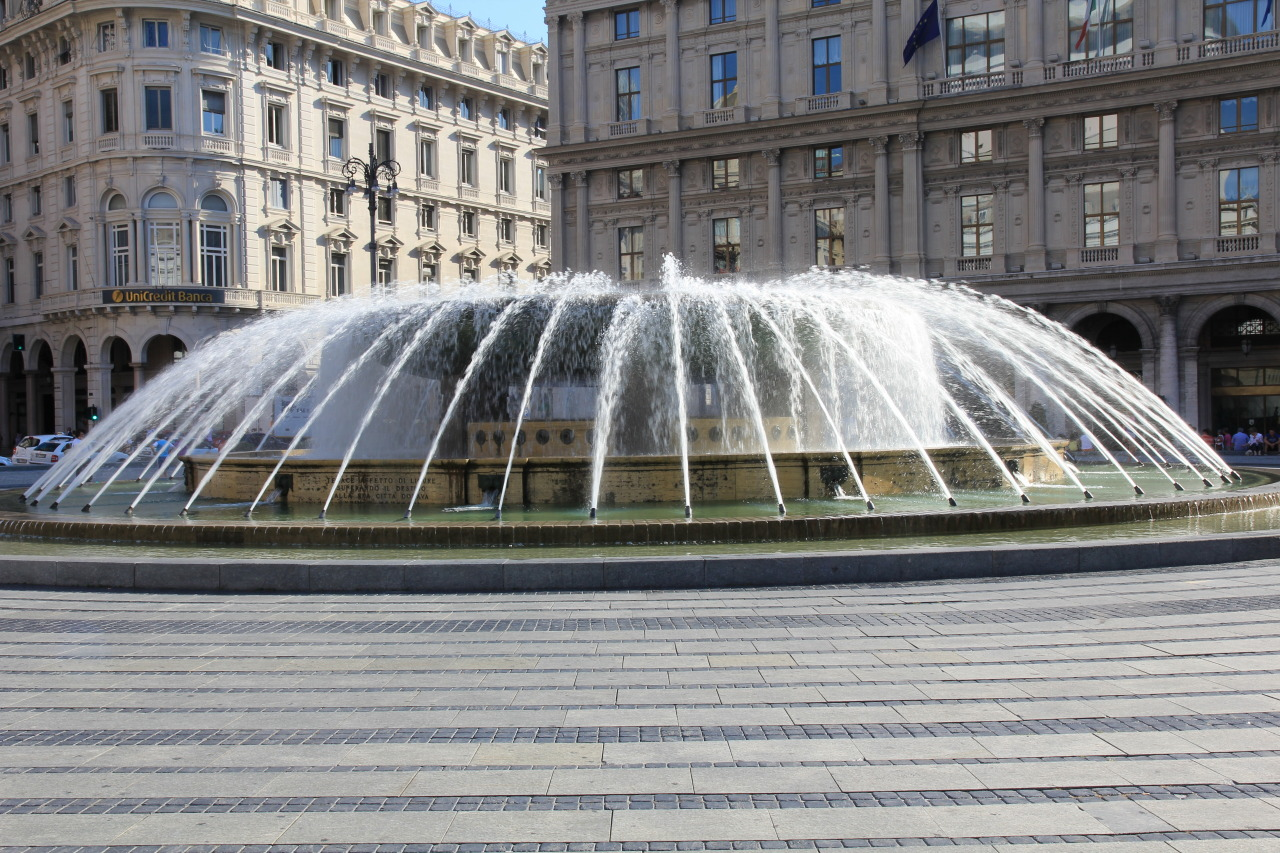
\includegraphics[width=0.4\textwidth, height=5cm, keepaspectratio]{../Bilder/Sardinien/1.jpg}
%    \caption{Regen}
%  \end{centering}
%\end{wrapfigure} 

%\begin{figure}[b]
%   \centering
%      %\subfloat[CAPTION]{BILDERCODE}\qquad
%   \subfloat{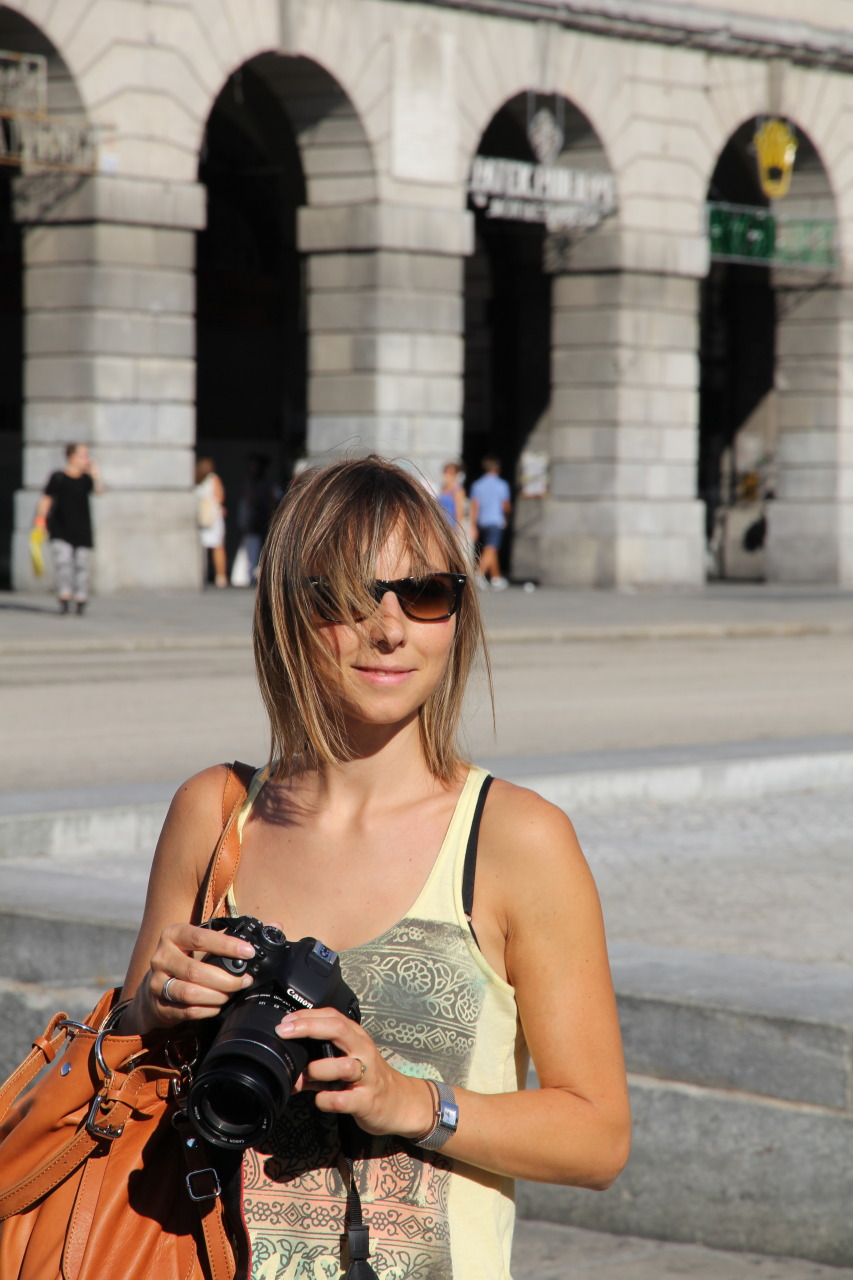
\includegraphics [width=0.3\textwidth]{../Bilder/Sardinien/2.jpg}}\quad
%   \subfloat{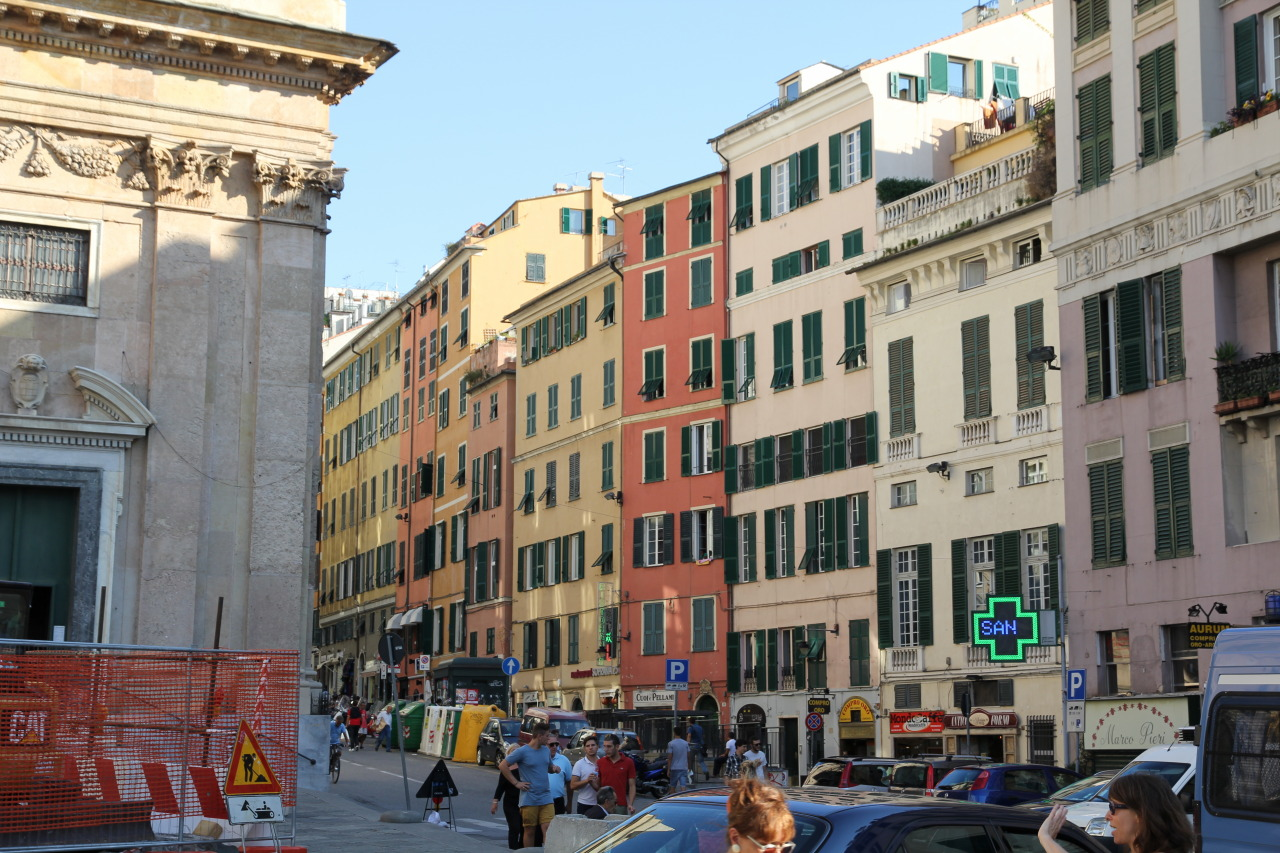
\includegraphics [width=0.3\textwidth]{../Bilder/Sardinien/3.jpg}}\quad
%   \subfloat{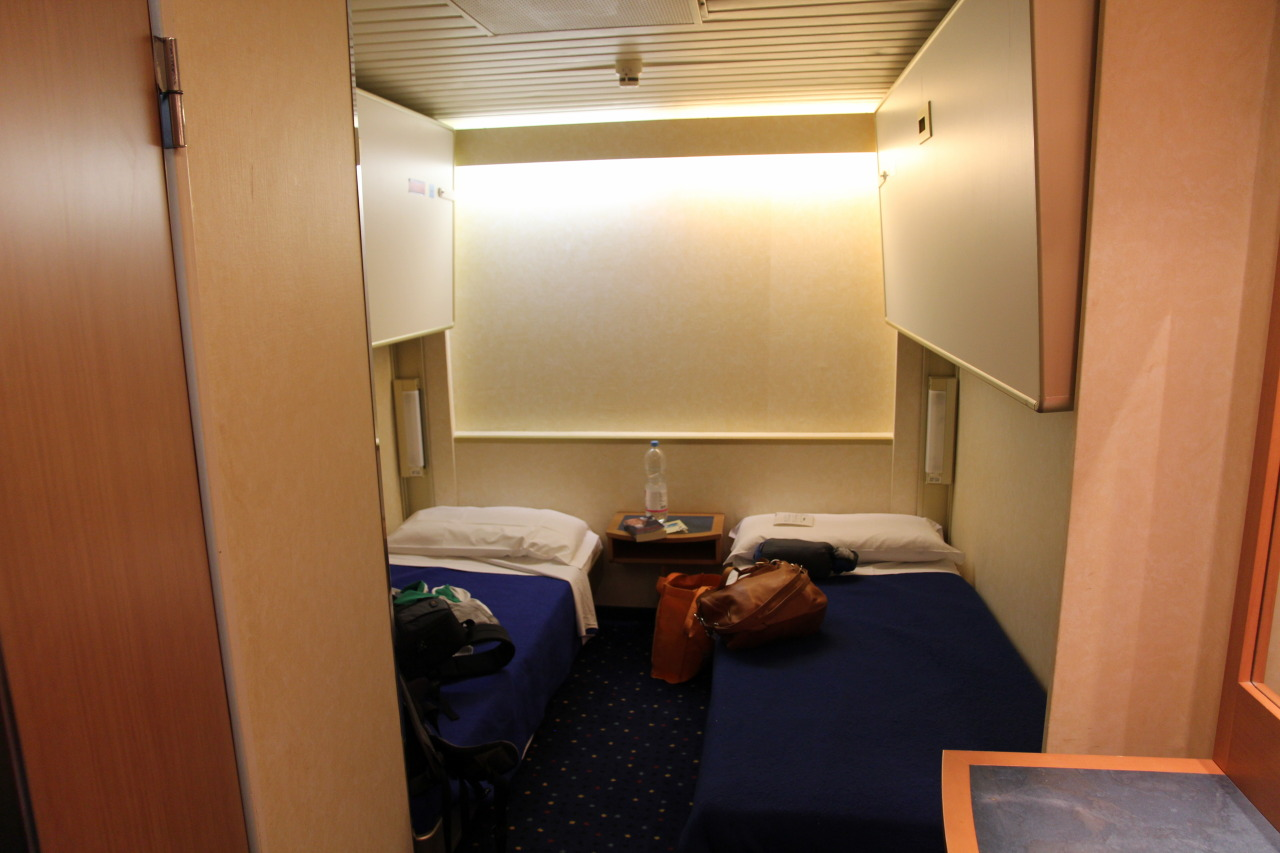
\includegraphics [width=0.3\textwidth]{../Bilder/Sardinien/4.jpg}}\quad
%   \caption[Meran]{Meran}
%\end{figure}

%\begin{figure}[hb]
%    \centering
%    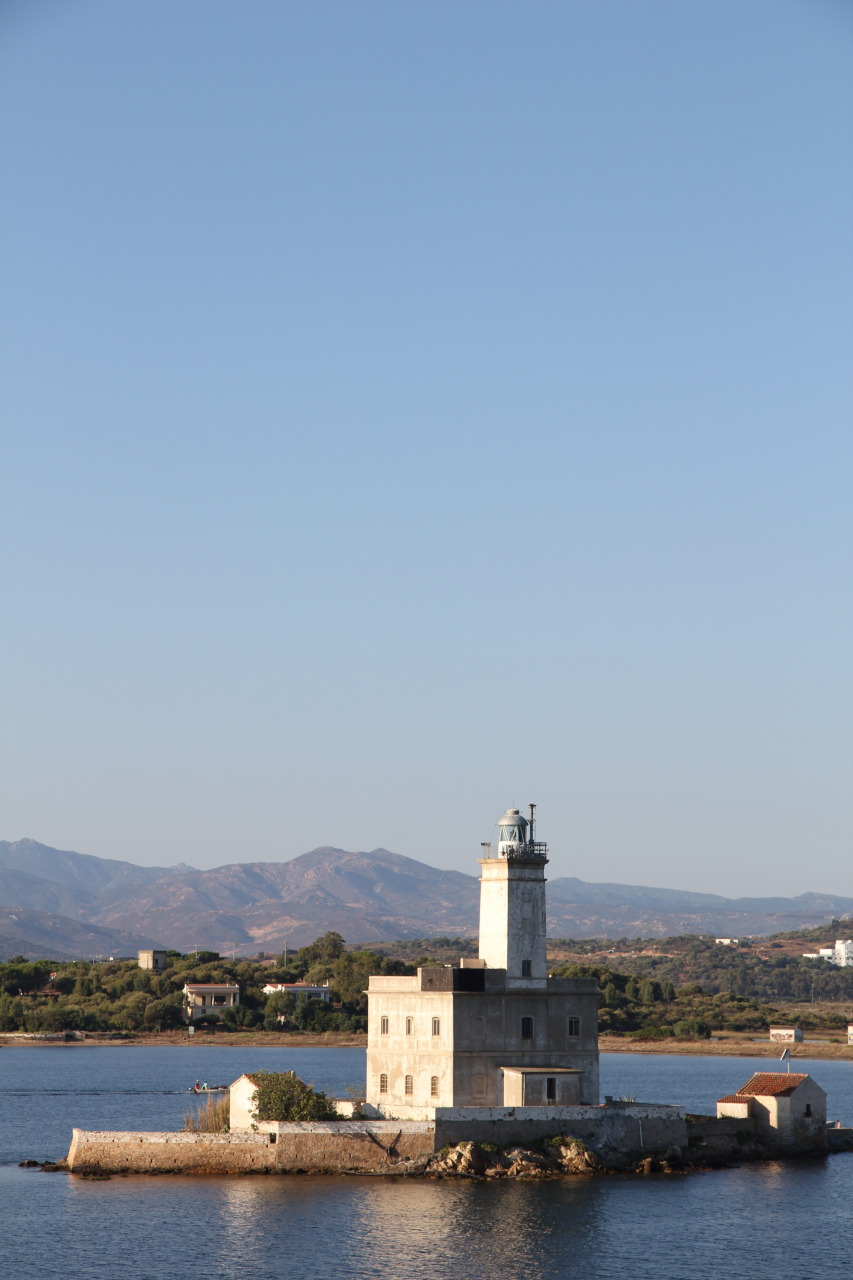
\includegraphics[width=\textwidth]{../Bilder/Sardinien/7.jpg}
%    \caption{Da sind sie ja...}
%    \label{img:Sardinien}
%\end{figure}

\subsection{Einleitung} 
Ein Geburtstag und eine damit verbundene Einladung lockte uns für einmal in den Norden.
Die Hitzewelle welche die Schweiz und Europa fest im Griff hatte lies von uns von tieferen Temperaturen träumen.
Eine zweiwöchige Geschäftsreise nach Phoenix mit Spitzentemperaturen von 47C erhöhten den Wunsch nach angenehmere Temperaturen nur noch mehr.
Das Ziel sollte Sylt sein.
Genauer gesagt Hörnum.
Da sich das Ziel doch über Tausend Kilometer entfernt befand wurde aus der Woche Ferien deren drei.
Eine Woche um in den Norden zu reisen, eine Woche auf Sylt und dann noch genügend Zeit um die Rückreise in den Süden anzutreten. 
Vor der Abfahrt sollte der Bus ein weiteres Mal für die lange Fahrt bereitgemacht werden.
Dieses Mal ging alles ganz Fix.
Die neuen Sitzüberzüge passten wie angegossen und werten den Innenraum merklich auf.

%\begin{wrapfigure}{R}{0.45\textwidth} 
%  \begin{centering}
%    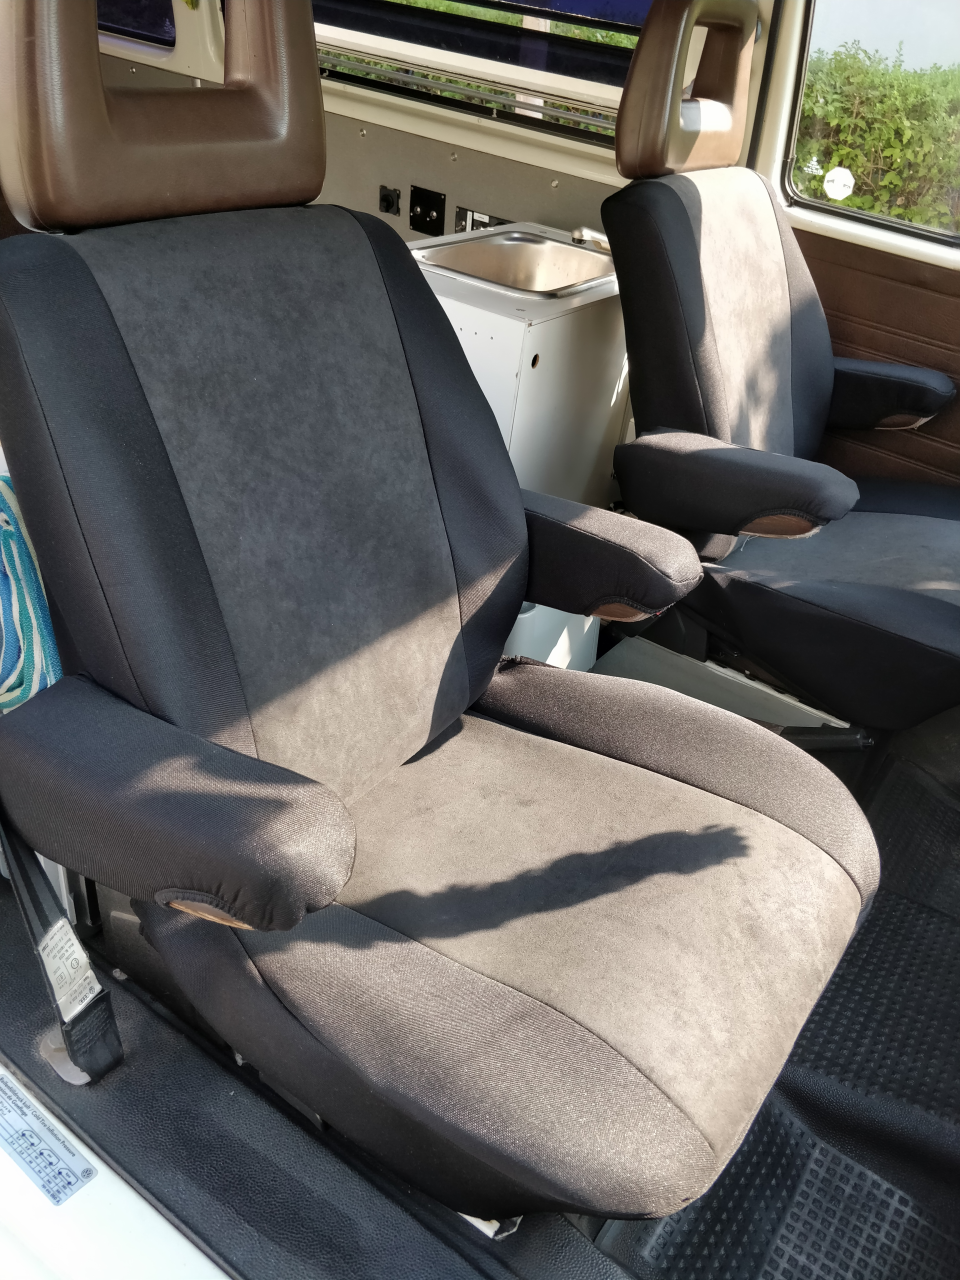
\includegraphics[width=0.4\textwidth, height=5cm, keepaspectratio]{../Bilder/Sylt/1.jpg}
%    \caption{Regen}
%  \end{centering}
%\end{wrapfigure} 

\subsection{06.08.2018 Heisse Fahrt in den Norden} 
Eigentlich war wollten wir schon am Samstag los. Ein Arzttermin machte uns jedoch einen Strich durch die Rechnung.
Die Ursache für den Arzttermin machte jedoch die Verspätung auf jeden Fall lohnenswert.
Also ging die Fahrt erst kurz nach drei los.
Wie vorhin schon erwähnt war es ziemlich warm.
Die fehlende Klimaanlage machte sich relativ schnell bemerkbar und erzeugte bei der Beifahrerin nicht gerade Freude.
Das erste Ziel sollte Heidelberg sein.
Warum?
Einfach so, liegt auf der Strecke und sollte innerhalb eines halben Tages gut erreichbar sein.
Nebenbei scheint es auch eine hübsche Stadt zu sein. 
Die kurze Google Bildersuche schien auf jeden Fall darauf hinzuweisen.
Zu guter Letzt hat es dort Wasser im Form der Necker, welche durch die Stadt fliesst.
Gerade bei den Temperaturen ein sehr gutes Argument.
Die Reise über Basel verlieg problemlos und nur mit geringem Stau.
Zwischendurch meinte das Navi die Distanz zum Ziel zwar zu verringern, die Zeit bis zum Ziel jedoch stetig ansteigen zu lassen.
Nicht gerade motivierend.
Bis wir jedoch das Stauende erreicht hatten war das Schlimmste schon längst vorbei.
Unterwegs wurde Kontakt mit einem Zeltplatz aufgenommen und es wurde bestätigt, dass die Reception bis um halb Neun offen sein sollte.
Kurz vor Acht trafen wir dann auf dem Campingplatz ein.
Absolut durchnässt von den hohen Temperaturen war die Dusche eine reine Wohltat.
